\documentclass[1p]{elsarticle_modified}
%\bibliographystyle{elsarticle-num}

%\usepackage[colorlinks]{hyperref}
%\usepackage{abbrmath_seonhwa} %\Abb, \Ascr, \Acal ,\Abf, \Afrak
\usepackage{amsfonts}
\usepackage{amssymb}
\usepackage{amsmath}
\usepackage{amsthm}
\usepackage{scalefnt}
\usepackage{amsbsy}
\usepackage{kotex}
\usepackage{caption}
\usepackage{subfig}
\usepackage{color}
\usepackage{graphicx}
\usepackage{xcolor} %% white, black, red, green, blue, cyan, magenta, yellow
\usepackage{float}
\usepackage{setspace}
\usepackage{hyperref}

\usepackage{tikz}
\usetikzlibrary{arrows}

\usepackage{multirow}
\usepackage{array} % fixed length table
\usepackage{hhline}

%%%%%%%%%%%%%%%%%%%%%
\makeatletter
\renewcommand*\env@matrix[1][\arraystretch]{%
	\edef\arraystretch{#1}%
	\hskip -\arraycolsep
	\let\@ifnextchar\new@ifnextchar
	\array{*\c@MaxMatrixCols c}}
\makeatother %https://tex.stackexchange.com/questions/14071/how-can-i-increase-the-line-spacing-in-a-matrix
%%%%%%%%%%%%%%%

\usepackage[normalem]{ulem}

\newcommand{\msout}[1]{\ifmmode\text{\sout{\ensuremath{#1}}}\else\sout{#1}\fi}
%SOURCE: \msout is \stkout macro in https://tex.stackexchange.com/questions/20609/strikeout-in-math-mode

\newcommand{\cancel}[1]{
	\ifmmode
	{\color{red}\msout{#1}}
	\else
	{\color{red}\sout{#1}}
	\fi
}

\newcommand{\add}[1]{
	{\color{blue}\uwave{#1}}
}

\newcommand{\replace}[2]{
	\ifmmode
	{\color{red}\msout{#1}}{\color{blue}\uwave{#2}}
	\else
	{\color{red}\sout{#1}}{\color{blue}\uwave{#2}}
	\fi
}

\newcommand{\Sol}{\mathcal{S}} %segment
\newcommand{\D}{D} %diagram
\newcommand{\A}{\mathcal{A}} %arc


%%%%%%%%%%%%%%%%%%%%%%%%%%%%%5 test

\def\sl{\operatorname{\textup{SL}}(2,\Cbb)}
\def\psl{\operatorname{\textup{PSL}}(2,\Cbb)}
\def\quan{\mkern 1mu \triangleright \mkern 1mu}

\theoremstyle{definition}
\newtheorem{thm}{Theorem}[section]
\newtheorem{prop}[thm]{Proposition}
\newtheorem{lem}[thm]{Lemma}
\newtheorem{ques}[thm]{Question}
\newtheorem{cor}[thm]{Corollary}
\newtheorem{defn}[thm]{Definition}
\newtheorem{exam}[thm]{Example}
\newtheorem{rmk}[thm]{Remark}
\newtheorem{alg}[thm]{Algorithm}

\newcommand{\I}{\sqrt{-1}}
\begin{document}

%\begin{frontmatter}
%
%\title{Boundary parabolic representations of knots up to 8 crossings}
%
%%% Group authors per affiliation:
%\author{Yunhi Cho} 
%\address{Department of Mathematics, University of Seoul, Seoul, Korea}
%\ead{yhcho@uos.ac.kr}
%
%
%\author{Seonhwa Kim} %\fnref{s_kim}}
%\address{Center for Geometry and Physics, Institute for Basic Science, Pohang, 37673, Korea}
%\ead{ryeona17@ibs.re.kr}
%
%\author{Hyuk Kim}
%\address{Department of Mathematical Sciences, Seoul National University, Seoul 08826, Korea}
%\ead{hyukkim@snu.ac.kr}
%
%\author{Seokbeom Yoon}
%\address{Department of Mathematical Sciences, Seoul National University, Seoul, 08826,  Korea}
%\ead{sbyoon15@snu.ac.kr}
%
%\begin{abstract}
%We find all boundary parabolic representation of knots up to 8 crossings.
%
%\end{abstract}
%\begin{keyword}
%    \MSC[2010] 57M25 
%\end{keyword}
%
%\end{frontmatter}

%\linenumbers
%\tableofcontents
%
\newcommand\colored[1]{\textcolor{white}{\rule[-0.35ex]{0.8em}{1.4ex}}\kern-0.8em\color{red} #1}%
%\newcommand\colored[1]{\textcolor{white}{ #1}\kern-2.17ex	\textcolor{white}{ #1}\kern-1.81ex	\textcolor{white}{ #1}\kern-2.15ex\color{red}#1	}

{\Large $\underline{11a_{318}~(K11a_{318})}$}

\setlength{\tabcolsep}{10pt}
\renewcommand{\arraystretch}{1.6}
\vspace{1cm}\begin{tabular}{m{100pt}>{\centering\arraybackslash}m{274pt}}
\multirow{5}{120pt}{
	\centering
	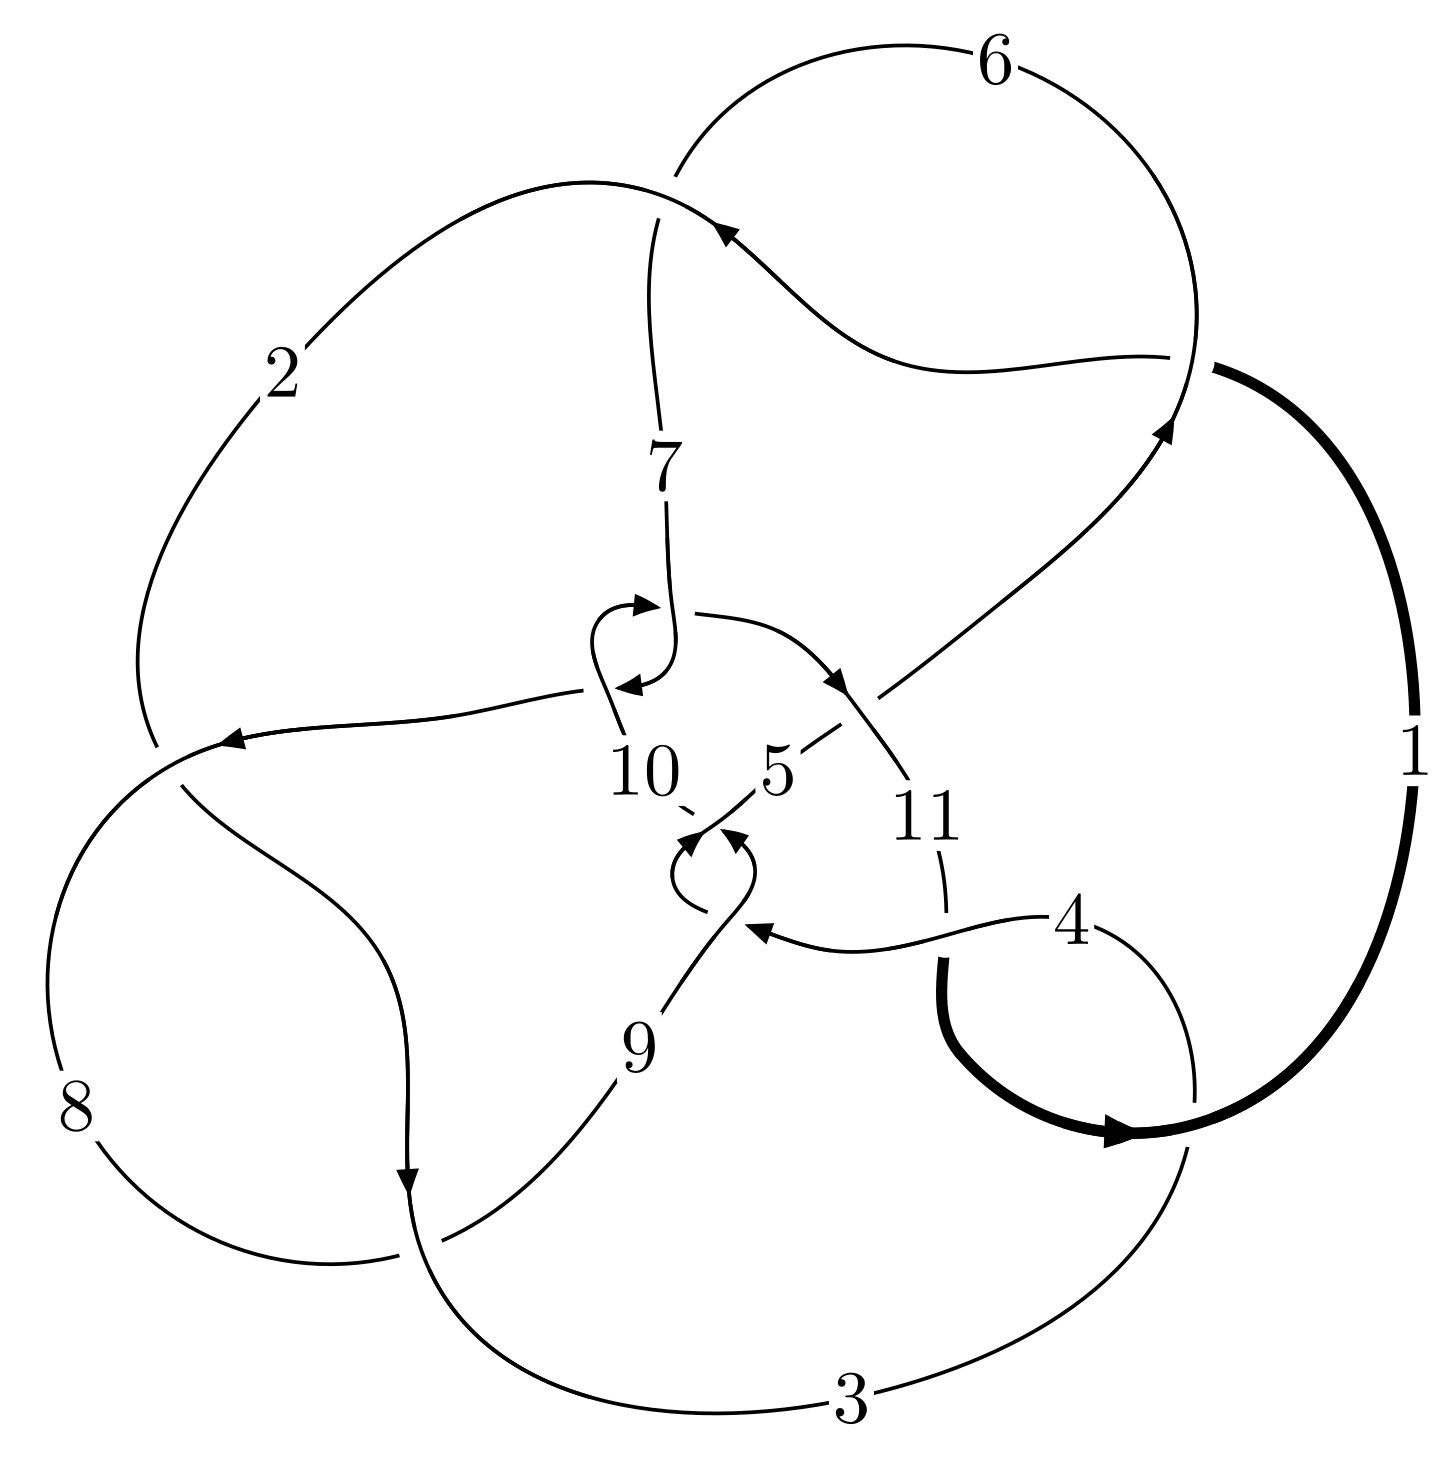
\includegraphics[width=112pt]{../../../GIT/diagram.site/Diagrams/png/567_11a_318.png}\\
\ \ \ A knot diagram\footnotemark}&
\allowdisplaybreaks
\textbf{Linearized knot diagam} \\
\cline{2-2}
 &
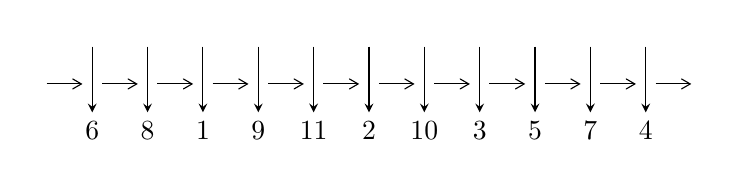
\begin{tikzpicture}[x=20pt, y=17pt]
	% nodes
	\node (C0) at (0, 0) {};
	\node (C1) at (1, 0) {};
	\node (C1U) at (1, +1) {};
	\node (C1D) at (1, -1) {6};

	\node (C2) at (2, 0) {};
	\node (C2U) at (2, +1) {};
	\node (C2D) at (2, -1) {8};

	\node (C3) at (3, 0) {};
	\node (C3U) at (3, +1) {};
	\node (C3D) at (3, -1) {1};

	\node (C4) at (4, 0) {};
	\node (C4U) at (4, +1) {};
	\node (C4D) at (4, -1) {9};

	\node (C5) at (5, 0) {};
	\node (C5U) at (5, +1) {};
	\node (C5D) at (5, -1) {11};

	\node (C6) at (6, 0) {};
	\node (C6U) at (6, +1) {};
	\node (C6D) at (6, -1) {2};

	\node (C7) at (7, 0) {};
	\node (C7U) at (7, +1) {};
	\node (C7D) at (7, -1) {10};

	\node (C8) at (8, 0) {};
	\node (C8U) at (8, +1) {};
	\node (C8D) at (8, -1) {3};

	\node (C9) at (9, 0) {};
	\node (C9U) at (9, +1) {};
	\node (C9D) at (9, -1) {5};

	\node (C10) at (10, 0) {};
	\node (C10U) at (10, +1) {};
	\node (C10D) at (10, -1) {7};

	\node (C11) at (11, 0) {};
	\node (C11U) at (11, +1) {};
	\node (C11D) at (11, -1) {4};
	\node (C12) at (12, 0) {};

	% arrows
	\draw[->,>={angle 60}]
	(C0) edge (C1) (C1) edge (C2) (C2) edge (C3) (C3) edge (C4) (C4) edge (C5) (C5) edge (C6) (C6) edge (C7) (C7) edge (C8) (C8) edge (C9) (C9) edge (C10) (C10) edge (C11) (C11) edge (C12) ;	\draw[->,>=stealth]
	(C1U) edge (C1D) (C2U) edge (C2D) (C3U) edge (C3D) (C4U) edge (C4D) (C5U) edge (C5D) (C6U) edge (C6D) (C7U) edge (C7D) (C8U) edge (C8D) (C9U) edge (C9D) (C10U) edge (C10D) (C11U) edge (C11D) ;
	\end{tikzpicture} \\
\hhline{~~} \\& 
\textbf{Solving Sequence} \\ \cline{2-2} 
 &
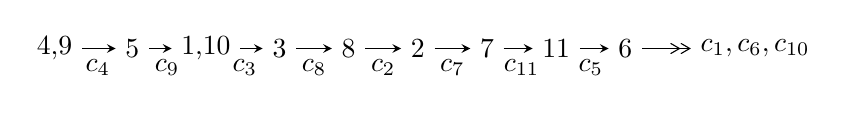
\begin{tikzpicture}[x=25pt, y=7pt]
	% node
	\node (A0) at (-1/8, 0) {4,9};
	\node (A1) at (1, 0) {5};
	\node (A2) at (33/16, 0) {1,10};
	\node (A3) at (25/8, 0) {3};
	\node (A4) at (33/8, 0) {8};
	\node (A5) at (41/8, 0) {2};
	\node (A6) at (49/8, 0) {7};
	\node (A7) at (57/8, 0) {11};
	\node (A8) at (65/8, 0) {6};
	\node (C1) at (1/2, -1) {$c_{4}$};
	\node (C2) at (3/2, -1) {$c_{9}$};
	\node (C3) at (21/8, -1) {$c_{3}$};
	\node (C4) at (29/8, -1) {$c_{8}$};
	\node (C5) at (37/8, -1) {$c_{2}$};
	\node (C6) at (45/8, -1) {$c_{7}$};
	\node (C7) at (53/8, -1) {$c_{11}$};
	\node (C8) at (61/8, -1) {$c_{5}$};
	\node (A9) at (10, 0) {$c_{1},c_{6},c_{10}$};

	% edge
	\draw[->,>=stealth]	
	(A0) edge (A1) (A1) edge (A2) (A2) edge (A3) (A3) edge (A4) (A4) edge (A5) (A5) edge (A6) (A6) edge (A7) (A7) edge (A8) ;
	\draw[->>,>={angle 60}]	
	(A8) edge (A9);
\end{tikzpicture} \\ 

\end{tabular} \\

\footnotetext{
The image of knot diagram is generated by the software ``\textbf{Draw programme}" developed by Andrew Bartholomew(\url{http://www.layer8.co.uk/maths/draw/index.htm\#Running-draw}), where we modified some parts for our purpose(\url{https://github.com/CATsTAILs/LinksPainter}).
}\phantom \\ \newline 
\centering \textbf{Ideals for irreducible components\footnotemark of $X_{\text{par}}$} 
 
\begin{align*}
I^u_{1}&=\langle 
970383 u^{17}+408499 u^{16}+\cdots+1982053 b+372351,\\
\phantom{I^u_{1}}&\phantom{= \langle  }-1777862 u^{17}-876895 u^{16}+\cdots+1982053 a-4101509,\;u^{18}+u^{17}+\cdots+u^2-1\rangle \\
I^u_{2}&=\langle 
7.25333\times10^{100} u^{59}+1.20321\times10^{99} u^{58}+\cdots+5.25066\times10^{101} b-1.15506\times10^{102},\\
\phantom{I^u_{2}}&\phantom{= \langle  }-3.92526\times10^{102} u^{59}+3.63473\times10^{101} u^{58}+\cdots+8.92612\times10^{102} a+1.52814\times10^{104},\\
\phantom{I^u_{2}}&\phantom{= \langle  }u^{60}- u^{59}+\cdots-109 u+17\rangle \\
I^u_{3}&=\langle 
-509 u^{19}-338 u^{18}+\cdots+367 b-1165,\;610 u^{19}-321 u^{18}+\cdots+367 a-671,\;u^{20}-8 u^{18}+\cdots+u-1\rangle \\
I^u_{4}&=\langle 
u^3+b+1,\;u^2+a+u,\;u^4+u-1\rangle \\
I^u_{5}&=\langle 
638 u^{11}-606 u^{10}+\cdots+697 b-1440,\;936 u^{11}+352 u^{10}+\cdots+697 a-1503,\\
\phantom{I^u_{5}}&\phantom{= \langle  }u^{12}-2 u^{10}+u^9-5 u^7+6 u^6+u^5-9 u^4+5 u^3+6 u^2-2 u-1\rangle \\
I^u_{6}&=\langle 
b+1,\;a+1,\;u-1\rangle \\
\\
\end{align*}
\raggedright * 6 irreducible components of $\dim_{\mathbb{C}}=0$, with total 115 representations.\\
\footnotetext{All coefficients of polynomials are rational numbers. But the coefficients are sometimes approximated in decimal forms when there is not enough margin.}
\newpage
\renewcommand{\arraystretch}{1}
\centering \section*{I. $I^u_{1}= \langle 9.70\times10^{5} u^{17}+4.08\times10^{5} u^{16}+\cdots+1.98\times10^{6} b+3.72\times10^{5},\;-1.78\times10^{6} u^{17}-8.77\times10^{5} u^{16}+\cdots+1.98\times10^{6} a-4.10\times10^{6},\;u^{18}+u^{17}+\cdots+u^2-1 \rangle$}
\flushleft \textbf{(i) Arc colorings}\\
\begin{tabular}{m{7pt} m{180pt} m{7pt} m{180pt} }
\flushright $a_{4}=$&$\begin{pmatrix}1\\0\end{pmatrix}$ \\
\flushright $a_{9}=$&$\begin{pmatrix}0\\u\end{pmatrix}$ \\
\flushright $a_{5}=$&$\begin{pmatrix}1\\u^2\end{pmatrix}$ \\
\flushright $a_{1}=$&$\begin{pmatrix}0.896980 u^{17}+0.442418 u^{16}+\cdots-1.43884 u+2.06932\\-0.489585 u^{17}-0.206099 u^{16}+\cdots+1.33228 u-0.187861\end{pmatrix}$ \\
\flushright $a_{10}=$&$\begin{pmatrix}- u\\- u^3+u\end{pmatrix}$ \\
\flushright $a_{3}=$&$\begin{pmatrix}0.0859684 u^{17}+0.537916 u^{16}+\cdots-8.56326 u+0.601597\\0.459466 u^{17}-0.352058 u^{16}+\cdots+1.86468 u+0.0670699\end{pmatrix}$ \\
\flushright $a_{8}=$&$\begin{pmatrix}0.799368 u^{17}+0.226871 u^{16}+\cdots-7.13272 u-2.24851\\0.229761 u^{17}+0.320704 u^{16}+\cdots+2.30647 u+0.343733\end{pmatrix}$ \\
\flushright $a_{2}=$&$\begin{pmatrix}0.139285 u^{17}+0.903251 u^{16}+\cdots-3.05848 u+3.34917\\0.00845336 u^{17}-0.364603 u^{16}+\cdots+1.75892 u-0.515882\end{pmatrix}$ \\
\flushright $a_{7}=$&$\begin{pmatrix}0.515882 u^{17}+0.507429 u^{16}+\cdots-6.94486 u-1.75892\\0.0450356 u^{17}+0.277375 u^{16}+\cdots+1.83513 u+0.418192\end{pmatrix}$ \\
\flushright $a_{11}=$&$\begin{pmatrix}0.407395 u^{17}+0.236319 u^{16}+\cdots-0.106565 u+1.88146\\-0.489585 u^{17}-0.206099 u^{16}+\cdots+1.33228 u-0.187861\end{pmatrix}$ \\
\flushright $a_{6}=$&$\begin{pmatrix}-1.27985 u^{17}-0.522154 u^{16}+\cdots+3.59568 u+1.61964\\0.328021 u^{17}-0.170017 u^{16}+\cdots-1.31924 u-0.426645\end{pmatrix}$\\ \flushright $a_{6}=$&$\begin{pmatrix}-1.27985 u^{17}-0.522154 u^{16}+\cdots+3.59568 u+1.61964\\0.328021 u^{17}-0.170017 u^{16}+\cdots-1.31924 u-0.426645\end{pmatrix}$\\&\end{tabular}
\flushleft \textbf{(ii) Obstruction class $= -1$}\\~\\
\flushleft \textbf{(iii) Cusp Shapes $= \frac{763801}{1982053} u^{17}+\frac{1992896}{1982053} u^{16}+\cdots+\frac{433836}{1982053} u-\frac{27209831}{1982053}$}\\~\\
\newpage\renewcommand{\arraystretch}{1}
\flushleft \textbf{(iv) u-Polynomials at the component}\newline \\
\begin{tabular}{m{50pt}|m{274pt}}
Crossings & \hspace{64pt}u-Polynomials at each crossing \\
\hline $$\begin{aligned}c_{1},c_{4},c_{6}\\c_{9}\end{aligned}$$&$\begin{aligned}
&u^{18}+u^{17}+\cdots+u^2-1
\end{aligned}$\\
\hline $$\begin{aligned}c_{2},c_{8}\end{aligned}$$&$\begin{aligned}
&u^{18}+u^{17}+\cdots+50 u+4
\end{aligned}$\\
\hline $$\begin{aligned}c_{3},c_{7},c_{10}\\c_{11}\end{aligned}$$&$\begin{aligned}
&u^{18}-2 u^{17}+\cdots+3 u+1
\end{aligned}$\\
\hline $$\begin{aligned}c_{5}\end{aligned}$$&$\begin{aligned}
&u^{18}+6 u^{17}+\cdots-416 u-64
\end{aligned}$\\
\hline
\end{tabular}\\~\\
\newpage\renewcommand{\arraystretch}{1}
\flushleft \textbf{(v) Riley Polynomials at the component}\newline \\
\begin{tabular}{m{50pt}|m{274pt}}
Crossings & \hspace{64pt}Riley Polynomials at each crossing \\
\hline $$\begin{aligned}c_{1},c_{4},c_{6}\\c_{9}\end{aligned}$$&$\begin{aligned}
&y^{18}-11 y^{17}+\cdots-2 y+1
\end{aligned}$\\
\hline $$\begin{aligned}c_{2},c_{8}\end{aligned}$$&$\begin{aligned}
&y^{18}-13 y^{17}+\cdots-1100 y+16
\end{aligned}$\\
\hline $$\begin{aligned}c_{3},c_{7},c_{10}\\c_{11}\end{aligned}$$&$\begin{aligned}
&y^{18}+8 y^{17}+\cdots-9 y+1
\end{aligned}$\\
\hline $$\begin{aligned}c_{5}\end{aligned}$$&$\begin{aligned}
&y^{18}+56 y^{16}+\cdots-37888 y+4096
\end{aligned}$\\
\hline
\end{tabular}\\~\\
\newpage\flushleft \textbf{(vi) Complex Volumes and Cusp Shapes}
$$\begin{array}{c|c|c}  
\text{Solutions to }I^u_{1}& \I (\text{vol} + \sqrt{-1}CS) & \text{Cusp shape}\\
 \hline 
\begin{aligned}
u &= \phantom{-}0.969317\phantom{ +0.000000I} \\
a &= -1.04231\phantom{ +0.000000I} \\
b &= -1.08420\phantom{ +0.000000I}\end{aligned}
 & -4.93604\phantom{ +0.000000I} & -18.1160\phantom{ +0.000000I} \\ \hline\begin{aligned}
u &= \phantom{-}0.503027 + 0.934053 I \\
a &= \phantom{-}0.117406 + 1.399640 I \\
b &= \phantom{-}0.129111 - 1.119030 I\end{aligned}
 & \phantom{-}5.93090 - 0.43570 I & -2.98328 + 1.68118 I \\ \hline\begin{aligned}
u &= \phantom{-}0.503027 - 0.934053 I \\
a &= \phantom{-}0.117406 - 1.399640 I \\
b &= \phantom{-}0.129111 + 1.119030 I\end{aligned}
 & \phantom{-}5.93090 + 0.43570 I & -2.98328 - 1.68118 I \\ \hline\begin{aligned}
u &= -1.155400 + 0.382844 I \\
a &= -0.0504197 - 0.0044892 I \\
b &= \phantom{-}1.25719 + 0.67749 I\end{aligned}
 & -8.49225 + 3.12657 I & -16.5106 - 4.5687 I \\ \hline\begin{aligned}
u &= -1.155400 - 0.382844 I \\
a &= -0.0504197 + 0.0044892 I \\
b &= \phantom{-}1.25719 - 0.67749 I\end{aligned}
 & -8.49225 - 3.12657 I & -16.5106 + 4.5687 I \\ \hline\begin{aligned}
u &= -1.219630 + 0.122646 I \\
a &= \phantom{-}1.35114 + 1.57540 I \\
b &= \phantom{-}0.417269 - 0.993577 I\end{aligned}
 & -4.77876 + 5.57099 I & -14.6445 - 6.8943 I \\ \hline\begin{aligned}
u &= -1.219630 - 0.122646 I \\
a &= \phantom{-}1.35114 - 1.57540 I \\
b &= \phantom{-}0.417269 + 0.993577 I\end{aligned}
 & -4.77876 - 5.57099 I & -14.6445 + 6.8943 I \\ \hline\begin{aligned}
u &= \phantom{-}1.306390 + 0.030156 I \\
a &= -0.314125 - 0.649221 I \\
b &= \phantom{-}0.308458 - 0.604810 I\end{aligned}
 & -7.41832 + 1.14356 I & -14.7481 - 6.1062 I \\ \hline\begin{aligned}
u &= \phantom{-}1.306390 - 0.030156 I \\
a &= -0.314125 + 0.649221 I \\
b &= \phantom{-}0.308458 + 0.604810 I\end{aligned}
 & -7.41832 - 1.14356 I & -14.7481 + 6.1062 I \\ \hline\begin{aligned}
u &= -1.244330 + 0.432653 I \\
a &= -1.32213 - 0.57859 I \\
b &= -0.507053 + 1.110690 I\end{aligned}
 & \phantom{-}0.46162 + 9.59091 I & -11.3598 - 8.6982 I\\
 \hline 
 \end{array}$$\newpage$$\begin{array}{c|c|c}  
\text{Solutions to }I^u_{1}& \I (\text{vol} + \sqrt{-1}CS) & \text{Cusp shape}\\
 \hline 
\begin{aligned}
u &= -1.244330 - 0.432653 I \\
a &= -1.32213 + 0.57859 I \\
b &= -0.507053 - 1.110690 I\end{aligned}
 & \phantom{-}0.46162 - 9.59091 I & -11.3598 + 8.6982 I \\ \hline\begin{aligned}
u &= -0.52847 + 1.35181 I \\
a &= \phantom{-}0.436864 + 1.177610 I \\
b &= -0.402613 - 0.935090 I\end{aligned}
 & \phantom{-}2.78527 - 3.16569 I & -11.24611 + 7.60453 I \\ \hline\begin{aligned}
u &= -0.52847 - 1.35181 I \\
a &= \phantom{-}0.436864 - 1.177610 I \\
b &= -0.402613 + 0.935090 I\end{aligned}
 & \phantom{-}2.78527 + 3.16569 I & -11.24611 - 7.60453 I \\ \hline\begin{aligned}
u &= \phantom{-}1.37244 + 0.65413 I \\
a &= \phantom{-}0.72292 - 1.23621 I \\
b &= \phantom{-}0.73238 + 1.24612 I\end{aligned}
 & -3.9350 - 17.2773 I & -12.8790 + 9.3490 I \\ \hline\begin{aligned}
u &= \phantom{-}1.37244 - 0.65413 I \\
a &= \phantom{-}0.72292 + 1.23621 I \\
b &= \phantom{-}0.73238 - 1.24612 I\end{aligned}
 & -3.9350 + 17.2773 I & -12.8790 - 9.3490 I \\ \hline\begin{aligned}
u &= -0.333926\phantom{ +0.000000I} \\
a &= \phantom{-}0.701030\phantom{ +0.000000I} \\
b &= -0.239136\phantom{ +0.000000I}\end{aligned}
 & -0.538352\phantom{ +0.000000I} & -18.5400\phantom{ +0.000000I} \\ \hline\begin{aligned}
u &= \phantom{-}0.148267 + 0.251923 I \\
a &= \phantom{-}3.22899 - 2.73957 I \\
b &= -0.273082 + 0.887649 I\end{aligned}
 & \phantom{-}1.73441 + 2.46344 I & -11.30045 - 4.80762 I \\ \hline\begin{aligned}
u &= \phantom{-}0.148267 - 0.251923 I \\
a &= \phantom{-}3.22899 + 2.73957 I \\
b &= -0.273082 - 0.887649 I\end{aligned}
 & \phantom{-}1.73441 - 2.46344 I & -11.30045 + 4.80762 I\\
 \hline 
 \end{array}$$\newpage\newpage\renewcommand{\arraystretch}{1}
\centering \section*{II. $I^u_{2}= \langle 7.25\times10^{100} u^{59}+1.20\times10^{99} u^{58}+\cdots+5.25\times10^{101} b-1.16\times10^{102},\;-3.93\times10^{102} u^{59}+3.63\times10^{101} u^{58}+\cdots+8.93\times10^{102} a+1.53\times10^{104},\;u^{60}- u^{59}+\cdots-109 u+17 \rangle$}
\flushleft \textbf{(i) Arc colorings}\\
\begin{tabular}{m{7pt} m{180pt} m{7pt} m{180pt} }
\flushright $a_{4}=$&$\begin{pmatrix}1\\0\end{pmatrix}$ \\
\flushright $a_{9}=$&$\begin{pmatrix}0\\u\end{pmatrix}$ \\
\flushright $a_{5}=$&$\begin{pmatrix}1\\u^2\end{pmatrix}$ \\
\flushright $a_{1}=$&$\begin{pmatrix}0.439749 u^{59}-0.0407201 u^{58}+\cdots+31.2675 u-17.1199\\-0.138141 u^{59}-0.00229154 u^{58}+\cdots-8.07888 u+2.19983\end{pmatrix}$ \\
\flushright $a_{10}=$&$\begin{pmatrix}- u\\- u^3+u\end{pmatrix}$ \\
\flushright $a_{3}=$&$\begin{pmatrix}-0.106939 u^{59}+0.0813048 u^{58}+\cdots+0.961685 u+8.85949\\-0.0242627 u^{59}+0.0260886 u^{58}+\cdots-2.48933 u-0.0619791\end{pmatrix}$ \\
\flushright $a_{8}=$&$\begin{pmatrix}-0.0488347 u^{59}-0.0246562 u^{58}+\cdots+10.6648 u+7.45876\\-0.144743 u^{59}-0.00850452 u^{58}+\cdots-13.1254 u+2.03107\end{pmatrix}$ \\
\flushright $a_{2}=$&$\begin{pmatrix}-0.254240 u^{59}-0.0726928 u^{58}+\cdots-28.4567 u+3.38184\\-0.312091 u^{59}+0.0424687 u^{58}+\cdots-33.3786 u+6.15466\end{pmatrix}$ \\
\flushright $a_{7}=$&$\begin{pmatrix}-0.141036 u^{59}-0.0530891 u^{58}+\cdots+1.08963 u+9.25438\\-0.159476 u^{59}+0.00805005 u^{58}+\cdots-15.1320 u+2.28623\end{pmatrix}$ \\
\flushright $a_{11}=$&$\begin{pmatrix}0.301608 u^{59}-0.0430116 u^{58}+\cdots+23.1886 u-14.9200\\-0.138141 u^{59}-0.00229154 u^{58}+\cdots-8.07888 u+2.19983\end{pmatrix}$ \\
\flushright $a_{6}=$&$\begin{pmatrix}-0.451448 u^{59}+0.0218306 u^{58}+\cdots-41.4070 u-0.151128\\0.0195413 u^{59}+0.0319909 u^{58}+\cdots+2.12465 u+0.466720\end{pmatrix}$\\ \flushright $a_{6}=$&$\begin{pmatrix}-0.451448 u^{59}+0.0218306 u^{58}+\cdots-41.4070 u-0.151128\\0.0195413 u^{59}+0.0319909 u^{58}+\cdots+2.12465 u+0.466720\end{pmatrix}$\\&\end{tabular}
\flushleft \textbf{(ii) Obstruction class $= -1$}\\~\\
\flushleft \textbf{(iii) Cusp Shapes $= 0.457112 u^{59}+0.104838 u^{58}+\cdots+36.7319 u-21.5900$}\\~\\
\newpage\renewcommand{\arraystretch}{1}
\flushleft \textbf{(iv) u-Polynomials at the component}\newline \\
\begin{tabular}{m{50pt}|m{274pt}}
Crossings & \hspace{64pt}u-Polynomials at each crossing \\
\hline $$\begin{aligned}c_{1},c_{4},c_{6}\\c_{9}\end{aligned}$$&$\begin{aligned}
&u^{60}- u^{59}+\cdots-109 u+17
\end{aligned}$\\
\hline $$\begin{aligned}c_{2},c_{8}\end{aligned}$$&$\begin{aligned}
&(u^{30}+6 u^{29}+\cdots+170 u+36)^{2}
\end{aligned}$\\
\hline $$\begin{aligned}c_{3},c_{7},c_{10}\\c_{11}\end{aligned}$$&$\begin{aligned}
&u^{60}-2 u^{59}+\cdots+2 u-1
\end{aligned}$\\
\hline $$\begin{aligned}c_{5}\end{aligned}$$&$\begin{aligned}
&(u^{30}-2 u^{29}+\cdots+2 u-1)^{2}
\end{aligned}$\\
\hline
\end{tabular}\\~\\
\newpage\renewcommand{\arraystretch}{1}
\flushleft \textbf{(v) Riley Polynomials at the component}\newline \\
\begin{tabular}{m{50pt}|m{274pt}}
Crossings & \hspace{64pt}Riley Polynomials at each crossing \\
\hline $$\begin{aligned}c_{1},c_{4},c_{6}\\c_{9}\end{aligned}$$&$\begin{aligned}
&y^{60}-41 y^{59}+\cdots-18409 y+289
\end{aligned}$\\
\hline $$\begin{aligned}c_{2},c_{8}\end{aligned}$$&$\begin{aligned}
&(y^{30}-22 y^{29}+\cdots-460 y+1296)^{2}
\end{aligned}$\\
\hline $$\begin{aligned}c_{3},c_{7},c_{10}\\c_{11}\end{aligned}$$&$\begin{aligned}
&y^{60}+32 y^{59}+\cdots+20 y+1
\end{aligned}$\\
\hline $$\begin{aligned}c_{5}\end{aligned}$$&$\begin{aligned}
&(y^{30}-2 y^{29}+\cdots-84 y+1)^{2}
\end{aligned}$\\
\hline
\end{tabular}\\~\\
\newpage\flushleft \textbf{(vi) Complex Volumes and Cusp Shapes}
$$\begin{array}{c|c|c}  
\text{Solutions to }I^u_{2}& \I (\text{vol} + \sqrt{-1}CS) & \text{Cusp shape}\\
 \hline 
\begin{aligned}
u &= -0.173863 + 0.983906 I \\
a &= -0.595302 - 1.227680 I \\
b &= \phantom{-}0.568581 + 1.096680 I\end{aligned}
 & -3.15719 - 4.84917 I & -13.58414 + 3.73183 I \\ \hline\begin{aligned}
u &= -0.173863 - 0.983906 I \\
a &= -0.595302 + 1.227680 I \\
b &= \phantom{-}0.568581 - 1.096680 I\end{aligned}
 & -3.15719 + 4.84917 I & -13.58414 - 3.73183 I \\ \hline\begin{aligned}
u &= -0.884656 + 0.446724 I \\
a &= -0.96473 - 1.07896 I \\
b &= -0.529022 - 0.052524 I\end{aligned}
 & -2.06368 + 5.36613 I & -15.7641 - 4.3359 I \\ \hline\begin{aligned}
u &= -0.884656 - 0.446724 I \\
a &= -0.96473 + 1.07896 I \\
b &= -0.529022 + 0.052524 I\end{aligned}
 & -2.06368 - 5.36613 I & -15.7641 + 4.3359 I \\ \hline\begin{aligned}
u &= -0.952526 + 0.271233 I \\
a &= -0.835395 + 0.173435 I \\
b &= -0.615493 + 0.932690 I\end{aligned}
 & \phantom{-}1.57409 + 1.75671 I & -11.26354 - 2.48942 I \\ \hline\begin{aligned}
u &= -0.952526 - 0.271233 I \\
a &= -0.835395 - 0.173435 I \\
b &= -0.615493 - 0.932690 I\end{aligned}
 & \phantom{-}1.57409 - 1.75671 I & -11.26354 + 2.48942 I \\ \hline\begin{aligned}
u &= \phantom{-}0.903459 + 0.213520 I \\
a &= -0.143616 + 1.243570 I \\
b &= -0.06489 - 1.61687 I\end{aligned}
 & \phantom{-}1.72325 - 5.82388 I & -14.0227 + 8.3964 I \\ \hline\begin{aligned}
u &= \phantom{-}0.903459 - 0.213520 I \\
a &= -0.143616 - 1.243570 I \\
b &= -0.06489 + 1.61687 I\end{aligned}
 & \phantom{-}1.72325 + 5.82388 I & -14.0227 - 8.3964 I \\ \hline\begin{aligned}
u &= \phantom{-}0.918123 + 0.113673 I \\
a &= \phantom{-}1.29720 - 2.26960 I \\
b &= \phantom{-}0.430781 + 1.048900 I\end{aligned}
 & -5.82415 - 2.23290 I & -14.1085 - 2.1221 I \\ \hline\begin{aligned}
u &= \phantom{-}0.918123 - 0.113673 I \\
a &= \phantom{-}1.29720 + 2.26960 I \\
b &= \phantom{-}0.430781 - 1.048900 I\end{aligned}
 & -5.82415 + 2.23290 I & -14.1085 + 2.1221 I\\
 \hline 
 \end{array}$$\newpage$$\begin{array}{c|c|c}  
\text{Solutions to }I^u_{2}& \I (\text{vol} + \sqrt{-1}CS) & \text{Cusp shape}\\
 \hline 
\begin{aligned}
u &= -1.058310 + 0.321731 I \\
a &= \phantom{-}0.993888 + 0.573737 I \\
b &= \phantom{-}0.319807 - 0.896497 I\end{aligned}
 & -0.48113 + 1.41291 I & -11.00000 + 0. I\phantom{ +0.000000I} \\ \hline\begin{aligned}
u &= -1.058310 - 0.321731 I \\
a &= \phantom{-}0.993888 - 0.573737 I \\
b &= \phantom{-}0.319807 + 0.896497 I\end{aligned}
 & -0.48113 - 1.41291 I & -11.00000 + 0. I\phantom{ +0.000000I} \\ \hline\begin{aligned}
u &= -0.868439 + 0.693479 I \\
a &= \phantom{-}0.592584 + 0.822702 I \\
b &= -0.315851 - 1.166500 I\end{aligned}
 & \phantom{-}1.57409 + 1.75671 I & -11.00000 + 0. I\phantom{ +0.000000I} \\ \hline\begin{aligned}
u &= -0.868439 - 0.693479 I \\
a &= \phantom{-}0.592584 - 0.822702 I \\
b &= -0.315851 + 1.166500 I\end{aligned}
 & \phantom{-}1.57409 - 1.75671 I & -11.00000 + 0. I\phantom{ +0.000000I} \\ \hline\begin{aligned}
u &= -0.172475 + 0.855408 I \\
a &= -0.33105 - 1.48907 I \\
b &= \phantom{-}0.616890 + 0.324785 I\end{aligned}
 & -2.27554 + 5.83321 I & -13.60048 - 3.60394 I \\ \hline\begin{aligned}
u &= -0.172475 - 0.855408 I \\
a &= -0.33105 + 1.48907 I \\
b &= \phantom{-}0.616890 - 0.324785 I\end{aligned}
 & -2.27554 - 5.83321 I & -13.60048 + 3.60394 I \\ \hline\begin{aligned}
u &= -0.723442 + 0.483773 I \\
a &= -1.08899 - 1.57094 I \\
b &= -0.601195 + 1.083620 I\end{aligned}
 & \phantom{-}1.99201 + 3.02567 I & -9.17011 - 1.57690 I \\ \hline\begin{aligned}
u &= -0.723442 - 0.483773 I \\
a &= -1.08899 + 1.57094 I \\
b &= -0.601195 - 1.083620 I\end{aligned}
 & \phantom{-}1.99201 - 3.02567 I & -9.17011 + 1.57690 I \\ \hline\begin{aligned}
u &= \phantom{-}0.913487 + 0.729355 I \\
a &= \phantom{-}0.84143 - 1.18997 I \\
b &= \phantom{-}0.839696 + 0.905250 I\end{aligned}
 & \phantom{-}1.72325 - 5.82388 I & \phantom{-0.000000 } 0 \\ \hline\begin{aligned}
u &= \phantom{-}0.913487 - 0.729355 I \\
a &= \phantom{-}0.84143 + 1.18997 I \\
b &= \phantom{-}0.839696 - 0.905250 I\end{aligned}
 & \phantom{-}1.72325 + 5.82388 I & \phantom{-0.000000 } 0\\
 \hline 
 \end{array}$$\newpage$$\begin{array}{c|c|c}  
\text{Solutions to }I^u_{2}& \I (\text{vol} + \sqrt{-1}CS) & \text{Cusp shape}\\
 \hline 
\begin{aligned}
u &= \phantom{-}0.681546 + 0.443831 I \\
a &= \phantom{-}1.314210 - 0.385156 I \\
b &= \phantom{-}0.168505 + 1.140690 I\end{aligned}
 & \phantom{-}1.99201 + 3.02567 I & -9.17011 - 1.57690 I \\ \hline\begin{aligned}
u &= \phantom{-}0.681546 - 0.443831 I \\
a &= \phantom{-}1.314210 + 0.385156 I \\
b &= \phantom{-}0.168505 - 1.140690 I\end{aligned}
 & \phantom{-}1.99201 - 3.02567 I & -9.17011 + 1.57690 I \\ \hline\begin{aligned}
u &= \phantom{-}0.639831 + 0.484680 I \\
a &= \phantom{-}0.649950 - 0.261552 I \\
b &= \phantom{-}0.343005 - 0.289428 I\end{aligned}
 & \phantom{-}2.17471 - 2.01374 I & -7.73585 + 3.91188 I \\ \hline\begin{aligned}
u &= \phantom{-}0.639831 - 0.484680 I \\
a &= \phantom{-}0.649950 + 0.261552 I \\
b &= \phantom{-}0.343005 + 0.289428 I\end{aligned}
 & \phantom{-}2.17471 + 2.01374 I & -7.73585 - 3.91188 I \\ \hline\begin{aligned}
u &= \phantom{-}1.036460 + 0.711450 I \\
a &= \phantom{-}0.32156 - 1.74527 I \\
b &= \phantom{-}0.521860 + 1.024170 I\end{aligned}
 & -6.56195 - 4.20028 I & \phantom{-0.000000 } 0 \\ \hline\begin{aligned}
u &= \phantom{-}1.036460 - 0.711450 I \\
a &= \phantom{-}0.32156 + 1.74527 I \\
b &= \phantom{-}0.521860 - 1.024170 I\end{aligned}
 & -6.56195 + 4.20028 I & \phantom{-0.000000 } 0 \\ \hline\begin{aligned}
u &= \phantom{-}1.26027\phantom{ +0.000000I} \\
a &= -0.136432\phantom{ +0.000000I} \\
b &= -1.08341\phantom{ +0.000000I}\end{aligned}
 & -5.55198\phantom{ +0.000000I} & \phantom{-0.000000 } 0 \\ \hline\begin{aligned}
u &= -0.673649 + 0.289156 I \\
a &= -2.03586 - 1.79948 I \\
b &= -0.100294 - 0.250395 I\end{aligned}
 & -2.10401 + 5.43294 I & -16.4599 - 1.4390 I \\ \hline\begin{aligned}
u &= -0.673649 - 0.289156 I \\
a &= -2.03586 + 1.79948 I \\
b &= -0.100294 + 0.250395 I\end{aligned}
 & -2.10401 - 5.43294 I & -16.4599 + 1.4390 I \\ \hline\begin{aligned}
u &= -0.205467 + 0.686465 I \\
a &= -0.31789 + 1.74264 I \\
b &= -0.325811 - 1.261230 I\end{aligned}
 & \phantom{-}3.74729 - 5.28000 I & -5.18091 + 3.40493 I\\
 \hline 
 \end{array}$$\newpage$$\begin{array}{c|c|c}  
\text{Solutions to }I^u_{2}& \I (\text{vol} + \sqrt{-1}CS) & \text{Cusp shape}\\
 \hline 
\begin{aligned}
u &= -0.205467 - 0.686465 I \\
a &= -0.31789 - 1.74264 I \\
b &= -0.325811 + 1.261230 I\end{aligned}
 & \phantom{-}3.74729 + 5.28000 I & -5.18091 - 3.40493 I \\ \hline\begin{aligned}
u &= \phantom{-}1.260710 + 0.276157 I \\
a &= -0.837013 + 0.676075 I \\
b &= -0.599749 - 1.161530 I\end{aligned}
 & -2.06368 - 5.36613 I & \phantom{-0.000000 } 0 \\ \hline\begin{aligned}
u &= \phantom{-}1.260710 - 0.276157 I \\
a &= -0.837013 - 0.676075 I \\
b &= -0.599749 + 1.161530 I\end{aligned}
 & -2.06368 + 5.36613 I & \phantom{-0.000000 } 0 \\ \hline\begin{aligned}
u &= \phantom{-}0.185453 + 1.290280 I \\
a &= -0.326081 + 1.289900 I \\
b &= \phantom{-}0.552043 - 1.093600 I\end{aligned}
 & -0.13405 + 10.50230 I & \phantom{-0.000000 } 0 \\ \hline\begin{aligned}
u &= \phantom{-}0.185453 - 1.290280 I \\
a &= -0.326081 - 1.289900 I \\
b &= \phantom{-}0.552043 + 1.093600 I\end{aligned}
 & -0.13405 - 10.50230 I & \phantom{-0.000000 } 0 \\ \hline\begin{aligned}
u &= \phantom{-}1.157510 + 0.625695 I \\
a &= \phantom{-}1.029550 - 0.832056 I \\
b &= \phantom{-}0.403736 + 0.982366 I\end{aligned}
 & \phantom{-}3.74729 - 5.28000 I & \phantom{-0.000000 } 0 \\ \hline\begin{aligned}
u &= \phantom{-}1.157510 - 0.625695 I \\
a &= \phantom{-}1.029550 + 0.832056 I \\
b &= \phantom{-}0.403736 - 0.982366 I\end{aligned}
 & \phantom{-}3.74729 + 5.28000 I & \phantom{-0.000000 } 0 \\ \hline\begin{aligned}
u &= \phantom{-}1.292280 + 0.285538 I \\
a &= -0.858396 + 0.914234 I \\
b &= -0.583662 - 1.209510 I\end{aligned}
 & -2.10401 - 5.43294 I & \phantom{-0.000000 } 0 \\ \hline\begin{aligned}
u &= \phantom{-}1.292280 - 0.285538 I \\
a &= -0.858396 - 0.914234 I \\
b &= -0.583662 + 1.209510 I\end{aligned}
 & -2.10401 + 5.43294 I & \phantom{-0.000000 } 0 \\ \hline\begin{aligned}
u &= -0.335964 + 0.575378 I \\
a &= \phantom{-}0.270786 - 0.040171 I \\
b &= -0.749034 - 0.108799 I\end{aligned}
 & -0.48113 - 1.41291 I & -11.50731 + 0.65666 I\\
 \hline 
 \end{array}$$\newpage$$\begin{array}{c|c|c}  
\text{Solutions to }I^u_{2}& \I (\text{vol} + \sqrt{-1}CS) & \text{Cusp shape}\\
 \hline 
\begin{aligned}
u &= -0.335964 - 0.575378 I \\
a &= \phantom{-}0.270786 + 0.040171 I \\
b &= -0.749034 + 0.108799 I\end{aligned}
 & -0.48113 + 1.41291 I & -11.50731 - 0.65666 I \\ \hline\begin{aligned}
u &= -1.290140 + 0.372995 I \\
a &= \phantom{-}0.0208764 + 0.0986315 I \\
b &= -0.980371 - 0.207899 I\end{aligned}
 & -3.15719 + 4.84917 I & \phantom{-0.000000 } 0 \\ \hline\begin{aligned}
u &= -1.290140 - 0.372995 I \\
a &= \phantom{-}0.0208764 - 0.0986315 I \\
b &= -0.980371 + 0.207899 I\end{aligned}
 & -3.15719 - 4.84917 I & \phantom{-0.000000 } 0 \\ \hline\begin{aligned}
u &= -0.099098 + 0.640186 I \\
a &= \phantom{-}0.09004 - 1.81958 I \\
b &= -0.212959 + 1.109000 I\end{aligned}
 & \phantom{-}2.17471 + 2.01374 I & -7.73585 - 3.91188 I \\ \hline\begin{aligned}
u &= -0.099098 - 0.640186 I \\
a &= \phantom{-}0.09004 + 1.81958 I \\
b &= -0.212959 - 1.109000 I\end{aligned}
 & \phantom{-}2.17471 - 2.01374 I & -7.73585 + 3.91188 I \\ \hline\begin{aligned}
u &= \phantom{-}1.291760 + 0.455145 I \\
a &= -0.0309170 - 0.0318134 I \\
b &= \phantom{-}1.187980 - 0.445839 I\end{aligned}
 & -6.51599 - 10.49730 I & \phantom{-0.000000 } 0 \\ \hline\begin{aligned}
u &= \phantom{-}1.291760 - 0.455145 I \\
a &= -0.0309170 + 0.0318134 I \\
b &= \phantom{-}1.187980 + 0.445839 I\end{aligned}
 & -6.51599 + 10.49730 I & \phantom{-0.000000 } 0 \\ \hline\begin{aligned}
u &= \phantom{-}1.306830 + 0.465197 I \\
a &= -0.630886 + 1.147070 I \\
b &= -0.620144 - 1.216600 I\end{aligned}
 & -2.27554 - 5.83321 I & \phantom{-0.000000 } 0 \\ \hline\begin{aligned}
u &= \phantom{-}1.306830 - 0.465197 I \\
a &= -0.630886 - 1.147070 I \\
b &= -0.620144 + 1.216600 I\end{aligned}
 & -2.27554 + 5.83321 I & \phantom{-0.000000 } 0 \\ \hline\begin{aligned}
u &= -1.269270 + 0.579030 I \\
a &= \phantom{-}0.723396 + 1.171420 I \\
b &= \phantom{-}0.81690 - 1.22821 I\end{aligned}
 & -6.51599 + 10.49730 I & \phantom{-0.000000 } 0\\
 \hline 
 \end{array}$$\newpage$$\begin{array}{c|c|c}  
\text{Solutions to }I^u_{2}& \I (\text{vol} + \sqrt{-1}CS) & \text{Cusp shape}\\
 \hline 
\begin{aligned}
u &= -1.269270 - 0.579030 I \\
a &= \phantom{-}0.723396 - 1.171420 I \\
b &= \phantom{-}0.81690 + 1.22821 I\end{aligned}
 & -6.51599 - 10.49730 I & \phantom{-0.000000 } 0 \\ \hline\begin{aligned}
u &= \phantom{-}1.40424 + 0.40913 I \\
a &= -0.380784 + 0.192994 I \\
b &= \phantom{-}0.481225 - 0.576338 I\end{aligned}
 & -7.98335\phantom{ +0.000000I} & \phantom{-0.000000 } 0 \\ \hline\begin{aligned}
u &= \phantom{-}1.40424 - 0.40913 I \\
a &= -0.380784 - 0.192994 I \\
b &= \phantom{-}0.481225 + 0.576338 I\end{aligned}
 & -7.98335\phantom{ +0.000000I} & \phantom{-0.000000 } 0 \\ \hline\begin{aligned}
u &= -1.50639 + 0.03128 I \\
a &= \phantom{-}0.313720 + 0.382658 I \\
b &= \phantom{-}0.350132 + 0.706526 I\end{aligned}
 & -5.82415 + 2.23290 I & \phantom{-0.000000 } 0 \\ \hline\begin{aligned}
u &= -1.50639 - 0.03128 I \\
a &= \phantom{-}0.313720 - 0.382658 I \\
b &= \phantom{-}0.350132 - 0.706526 I\end{aligned}
 & -5.82415 - 2.23290 I & \phantom{-0.000000 } 0 \\ \hline\begin{aligned}
u &= -1.33093 + 0.72650 I \\
a &= -0.54342 - 1.31576 I \\
b &= -0.605352 + 1.216900 I\end{aligned}
 & -0.13405 + 10.50230 I & \phantom{-0.000000 } 0 \\ \hline\begin{aligned}
u &= -1.33093 - 0.72650 I \\
a &= -0.54342 + 1.31576 I \\
b &= -0.605352 - 1.216900 I\end{aligned}
 & -0.13405 - 10.50230 I & \phantom{-0.000000 } 0 \\ \hline\begin{aligned}
u &= -1.64506 + 0.30278 I \\
a &= -0.056451 - 0.315590 I \\
b &= \phantom{-}0.504888 + 0.670086 I\end{aligned}
 & -6.56195 - 4.20028 I & \phantom{-0.000000 } 0 \\ \hline\begin{aligned}
u &= -1.64506 - 0.30278 I \\
a &= -0.056451 + 0.315590 I \\
b &= \phantom{-}0.504888 - 0.670086 I\end{aligned}
 & -6.56195 + 4.20028 I & \phantom{-0.000000 } 0 \\ \hline\begin{aligned}
u &= \phantom{-}0.135724\phantom{ +0.000000I} \\
a &= -10.1813\phantom{ +0.000000I} \\
b &= \phantom{-}0.678987\phantom{ +0.000000I}\end{aligned}
 & -5.55198\phantom{ +0.000000I} & -15.3380\phantom{ +0.000000I}\\
 \hline 
 \end{array}$$\newpage\newpage\renewcommand{\arraystretch}{1}
\centering \section*{III. $I^u_{3}= \langle -509 u^{19}-338 u^{18}+\cdots+367 b-1165,\;610 u^{19}-321 u^{18}+\cdots+367 a-671,\;u^{20}-8 u^{18}+\cdots+u-1 \rangle$}
\flushleft \textbf{(i) Arc colorings}\\
\begin{tabular}{m{7pt} m{180pt} m{7pt} m{180pt} }
\flushright $a_{4}=$&$\begin{pmatrix}1\\0\end{pmatrix}$ \\
\flushright $a_{9}=$&$\begin{pmatrix}0\\u\end{pmatrix}$ \\
\flushright $a_{5}=$&$\begin{pmatrix}1\\u^2\end{pmatrix}$ \\
\flushright $a_{1}=$&$\begin{pmatrix}-1.66213 u^{19}+0.874659 u^{18}+\cdots-4.53951 u+1.82834\\1.38692 u^{19}+0.920981 u^{18}+\cdots+1.83379 u+3.17439\end{pmatrix}$ \\
\flushright $a_{10}=$&$\begin{pmatrix}- u\\- u^3+u\end{pmatrix}$ \\
\flushright $a_{3}=$&$\begin{pmatrix}-0.250681 u^{19}-0.681199 u^{18}+\cdots+1.98093 u-1.32425\\0.752044 u^{19}-0.956403 u^{18}+\cdots+5.05722 u+0.972752\end{pmatrix}$ \\
\flushright $a_{8}=$&$\begin{pmatrix}-0.594005 u^{19}-0.00544959 u^{18}+\cdots+0.367847 u-1.74659\\-0.681199 u^{19}-1.19891 u^{18}+\cdots+1.92643 u-1.25068\end{pmatrix}$ \\
\flushright $a_{2}=$&$\begin{pmatrix}0.594005 u^{19}-0.994550 u^{18}+\cdots+2.63215 u-0.253406\\1.34060 u^{19}+0.599455 u^{18}+\cdots+4.53678 u+4.12534\end{pmatrix}$ \\
\flushright $a_{7}=$&$\begin{pmatrix}-0.673025 u^{19}-1.02452 u^{18}+\cdots+1.15531 u-3.35967\\-0.675749 u^{19}-0.749319 u^{18}+\cdots+2.07902 u-0.656676\end{pmatrix}$ \\
\flushright $a_{11}=$&$\begin{pmatrix}-0.275204 u^{19}+1.79564 u^{18}+\cdots-2.70572 u+5.00272\\1.38692 u^{19}+0.920981 u^{18}+\cdots+1.83379 u+3.17439\end{pmatrix}$ \\
\flushright $a_{6}=$&$\begin{pmatrix}1.65668 u^{19}-1.32425 u^{18}+\cdots+3.38692 u-2.42234\\-1.35422 u^{19}-0.223433 u^{18}+\cdots-2.91826 u-2.61035\end{pmatrix}$\\ \flushright $a_{6}=$&$\begin{pmatrix}1.65668 u^{19}-1.32425 u^{18}+\cdots+3.38692 u-2.42234\\-1.35422 u^{19}-0.223433 u^{18}+\cdots-2.91826 u-2.61035\end{pmatrix}$\\&\end{tabular}
\flushleft \textbf{(ii) Obstruction class $= 1$}\\~\\
\flushleft \textbf{(iii) Cusp Shapes $= \frac{1598}{367} u^{19}-\frac{3955}{367} u^{18}+\cdots+\frac{8778}{367} u-\frac{10786}{367}$}\\~\\
\newpage\renewcommand{\arraystretch}{1}
\flushleft \textbf{(iv) u-Polynomials at the component}\newline \\
\begin{tabular}{m{50pt}|m{274pt}}
Crossings & \hspace{64pt}u-Polynomials at each crossing \\
\hline $$\begin{aligned}c_{1},c_{4}\end{aligned}$$&$\begin{aligned}
&u^{20}-8 u^{18}+\cdots+u-1
\end{aligned}$\\
\hline $$\begin{aligned}c_{2}\end{aligned}$$&$\begin{aligned}
&(u^{10}-5 u^8+8 u^6+4 u^5-6 u^4-3 u^3+3 u^2-1)^2
\end{aligned}$\\
\hline $$\begin{aligned}c_{3},c_{10}\end{aligned}$$&$\begin{aligned}
&u^{20}+3 u^{19}+\cdots-8 u^2-1
\end{aligned}$\\
\hline $$\begin{aligned}c_{5}\end{aligned}$$&$\begin{aligned}
&u^{20}+8 u^{14}-52 u^{12}-138 u^{10}+104 u^8+527 u^6+296 u^4-356 u^2-319
\end{aligned}$\\
\hline $$\begin{aligned}c_{6},c_{9}\end{aligned}$$&$\begin{aligned}
&u^{20}-8 u^{18}+\cdots- u-1
\end{aligned}$\\
\hline $$\begin{aligned}c_{7},c_{11}\end{aligned}$$&$\begin{aligned}
&u^{20}-3 u^{19}+\cdots-8 u^2-1
\end{aligned}$\\
\hline $$\begin{aligned}c_{8}\end{aligned}$$&$\begin{aligned}
&(u^{10}-5 u^8+8 u^6-4 u^5-6 u^4+3 u^3+3 u^2-1)^2
\end{aligned}$\\
\hline
\end{tabular}\\~\\
\newpage\renewcommand{\arraystretch}{1}
\flushleft \textbf{(v) Riley Polynomials at the component}\newline \\
\begin{tabular}{m{50pt}|m{274pt}}
Crossings & \hspace{64pt}Riley Polynomials at each crossing \\
\hline $$\begin{aligned}c_{1},c_{4},c_{6}\\c_{9}\end{aligned}$$&$\begin{aligned}
&y^{20}-16 y^{19}+\cdots-13 y+1
\end{aligned}$\\
\hline $$\begin{aligned}c_{2},c_{8}\end{aligned}$$&$\begin{aligned}
&(y^{10}-10 y^9+\cdots-6 y+1)^{2}
\end{aligned}$\\
\hline $$\begin{aligned}c_{3},c_{7},c_{10}\\c_{11}\end{aligned}$$&$\begin{aligned}
&y^{20}+13 y^{19}+\cdots+16 y+1
\end{aligned}$\\
\hline $$\begin{aligned}c_{5}\end{aligned}$$&$\begin{aligned}
&(y^{10}+8 y^7-52 y^6-138 y^5+104 y^4+527 y^3+296 y^2-356 y-319)^{2}
\end{aligned}$\\
\hline
\end{tabular}\\~\\
\newpage\flushleft \textbf{(vi) Complex Volumes and Cusp Shapes}
$$\begin{array}{c|c|c}  
\text{Solutions to }I^u_{3}& \I (\text{vol} + \sqrt{-1}CS) & \text{Cusp shape}\\
 \hline 
\begin{aligned}
u &= -1.006880 + 0.379394 I \\
a &= \phantom{-}0.71131 + 2.12605 I \\
b &= \phantom{-}0.406554 - 1.044110 I\end{aligned}
 & -5.60500 + 3.07077 I & -11.10306 - 5.53745 I \\ \hline\begin{aligned}
u &= -1.006880 - 0.379394 I \\
a &= \phantom{-}0.71131 - 2.12605 I \\
b &= \phantom{-}0.406554 + 1.044110 I\end{aligned}
 & -5.60500 - 3.07077 I & -11.10306 + 5.53745 I \\ \hline\begin{aligned}
u &= -0.307724 + 0.858449 I \\
a &= \phantom{-}0.579281 + 0.822097 I \\
b &= -0.301268 - 1.054370 I\end{aligned}
 & \phantom{-}3.58542\phantom{ +0.000000I} & -5.93598 + 0. I\phantom{ +0.000000I} \\ \hline\begin{aligned}
u &= -0.307724 - 0.858449 I \\
a &= \phantom{-}0.579281 - 0.822097 I \\
b &= -0.301268 + 1.054370 I\end{aligned}
 & \phantom{-}3.58542\phantom{ +0.000000I} & -5.93598 + 0. I\phantom{ +0.000000I} \\ \hline\begin{aligned}
u &= -1.005260 + 0.622930 I \\
a &= -0.917585 - 0.950908 I \\
b &= -0.723749 + 0.881883 I\end{aligned}
 & \phantom{-}2.31904 + 5.08447 I & -9.51292 - 2.92589 I \\ \hline\begin{aligned}
u &= -1.005260 - 0.622930 I \\
a &= -0.917585 + 0.950908 I \\
b &= -0.723749 - 0.881883 I\end{aligned}
 & \phantom{-}2.31904 - 5.08447 I & -9.51292 + 2.92589 I \\ \hline\begin{aligned}
u &= -0.543411 + 0.587321 I \\
a &= \phantom{-}0.318117 + 0.503113 I \\
b &= -0.424021 - 1.175640 I\end{aligned}
 & \phantom{-}3.51176\phantom{ +0.000000I} & -5.53076 + 0. I\phantom{ +0.000000I} \\ \hline\begin{aligned}
u &= -0.543411 - 0.587321 I \\
a &= \phantom{-}0.318117 - 0.503113 I \\
b &= -0.424021 + 1.175640 I\end{aligned}
 & \phantom{-}3.51176\phantom{ +0.000000I} & -5.53076 + 0. I\phantom{ +0.000000I} \\ \hline\begin{aligned}
u &= \phantom{-}0.641197 + 0.460705 I \\
a &= \phantom{-}1.60910 - 2.98924 I \\
b &= \phantom{-}0.265764 + 0.633820 I\end{aligned}
 & -1.76138 - 5.90098 I & -8.4456 + 11.9708 I \\ \hline\begin{aligned}
u &= \phantom{-}0.641197 - 0.460705 I \\
a &= \phantom{-}1.60910 + 2.98924 I \\
b &= \phantom{-}0.265764 - 0.633820 I\end{aligned}
 & -1.76138 + 5.90098 I & -8.4456 - 11.9708 I\\
 \hline 
 \end{array}$$\newpage$$\begin{array}{c|c|c}  
\text{Solutions to }I^u_{3}& \I (\text{vol} + \sqrt{-1}CS) & \text{Cusp shape}\\
 \hline 
\begin{aligned}
u &= \phantom{-}1.22178\phantom{ +0.000000I} \\
a &= -0.206592\phantom{ +0.000000I} \\
b &= -1.34573\phantom{ +0.000000I}\end{aligned}
 & -6.32941\phantom{ +0.000000I} & -27.2570\phantom{ +0.000000I} \\ \hline\begin{aligned}
u &= -0.721984\phantom{ +0.000000I} \\
a &= \phantom{-}2.63740\phantom{ +0.000000I} \\
b &= \phantom{-}0.842412\phantom{ +0.000000I}\end{aligned}
 & -6.32941\phantom{ +0.000000I} & -27.2570\phantom{ +0.000000I} \\ \hline\begin{aligned}
u &= \phantom{-}1.322280 + 0.225447 I \\
a &= -0.769082 + 0.973657 I \\
b &= -0.528515 - 1.268130 I\end{aligned}
 & -1.76138 - 5.90098 I & -8.4456 + 11.9708 I \\ \hline\begin{aligned}
u &= \phantom{-}1.322280 - 0.225447 I \\
a &= -0.769082 - 0.973657 I \\
b &= -0.528515 + 1.268130 I\end{aligned}
 & -1.76138 + 5.90098 I & -8.4456 - 11.9708 I \\ \hline\begin{aligned}
u &= -1.361800 + 0.242619 I \\
a &= -0.490712 + 0.349688 I \\
b &= \phantom{-}0.255308 + 0.676358 I\end{aligned}
 & -7.12244\phantom{ +0.000000I} & -10.15337 + 0. I\phantom{ +0.000000I} \\ \hline\begin{aligned}
u &= -1.361800 - 0.242619 I \\
a &= -0.490712 - 0.349688 I \\
b &= \phantom{-}0.255308 - 0.676358 I\end{aligned}
 & -7.12244\phantom{ +0.000000I} & -10.15337 + 0. I\phantom{ +0.000000I} \\ \hline\begin{aligned}
u &= \phantom{-}0.502690 + 0.120984 I \\
a &= \phantom{-}0.432595 + 0.041333 I \\
b &= -0.14840 - 1.42580 I\end{aligned}
 & \phantom{-}2.31904 - 5.08447 I & -9.51292 + 2.92589 I \\ \hline\begin{aligned}
u &= \phantom{-}0.502690 - 0.120984 I \\
a &= \phantom{-}0.432595 - 0.041333 I \\
b &= -0.14840 + 1.42580 I\end{aligned}
 & \phantom{-}2.31904 + 5.08447 I & -9.51292 - 2.92589 I \\ \hline\begin{aligned}
u &= \phantom{-}1.50902 + 0.12166 I \\
a &= -0.688432 - 0.075728 I \\
b &= -0.050017 - 0.545597 I\end{aligned}
 & -5.60500 + 3.07077 I & -11.10306 - 5.53745 I \\ \hline\begin{aligned}
u &= \phantom{-}1.50902 - 0.12166 I \\
a &= -0.688432 + 0.075728 I \\
b &= -0.050017 + 0.545597 I\end{aligned}
 & -5.60500 - 3.07077 I & -11.10306 + 5.53745 I\\
 \hline 
 \end{array}$$\newpage\newpage\renewcommand{\arraystretch}{1}
\centering \section*{IV. $I^u_{4}= \langle u^3+b+1,\;u^2+a+u,\;u^4+u-1 \rangle$}
\flushleft \textbf{(i) Arc colorings}\\
\begin{tabular}{m{7pt} m{180pt} m{7pt} m{180pt} }
\flushright $a_{4}=$&$\begin{pmatrix}1\\0\end{pmatrix}$ \\
\flushright $a_{9}=$&$\begin{pmatrix}0\\u\end{pmatrix}$ \\
\flushright $a_{5}=$&$\begin{pmatrix}1\\u^2\end{pmatrix}$ \\
\flushright $a_{1}=$&$\begin{pmatrix}- u^2- u\\- u^3-1\end{pmatrix}$ \\
\flushright $a_{10}=$&$\begin{pmatrix}- u\\- u^3+u\end{pmatrix}$ \\
\flushright $a_{3}=$&$\begin{pmatrix}- u\\- u^3- u^2-1\end{pmatrix}$ \\
\flushright $a_{8}=$&$\begin{pmatrix}u^3\\u+1\end{pmatrix}$ \\
\flushright $a_{2}=$&$\begin{pmatrix}- u^2\\-1\end{pmatrix}$ \\
\flushright $a_{7}=$&$\begin{pmatrix}u^3+1\\u^2+u\end{pmatrix}$ \\
\flushright $a_{11}=$&$\begin{pmatrix}- u^3- u^2- u-1\\- u^3-1\end{pmatrix}$ \\
\flushright $a_{6}=$&$\begin{pmatrix}1\\u^2\end{pmatrix}$\\ \flushright $a_{6}=$&$\begin{pmatrix}1\\u^2\end{pmatrix}$\\&\end{tabular}
\flushleft \textbf{(ii) Obstruction class $= 1$}\\~\\
\flushleft \textbf{(iii) Cusp Shapes $= 4 u^3-2 u^2+3 u-6$}\\~\\
\newpage\renewcommand{\arraystretch}{1}
\flushleft \textbf{(iv) u-Polynomials at the component}\newline \\
\begin{tabular}{m{50pt}|m{274pt}}
Crossings & \hspace{64pt}u-Polynomials at each crossing \\
\hline $$\begin{aligned}c_{1},c_{4}\end{aligned}$$&$\begin{aligned}
&u^4+u-1
\end{aligned}$\\
\hline $$\begin{aligned}c_{2}\end{aligned}$$&$\begin{aligned}
&u^4-2 u^2+u+1
\end{aligned}$\\
\hline $$\begin{aligned}c_{3},c_{10}\end{aligned}$$&$\begin{aligned}
&u^4+u^3-1
\end{aligned}$\\
\hline $$\begin{aligned}c_{5}\end{aligned}$$&$\begin{aligned}
&u^4
\end{aligned}$\\
\hline $$\begin{aligned}c_{6},c_{9}\end{aligned}$$&$\begin{aligned}
&u^4- u-1
\end{aligned}$\\
\hline $$\begin{aligned}c_{7},c_{11}\end{aligned}$$&$\begin{aligned}
&u^4- u^3-1
\end{aligned}$\\
\hline $$\begin{aligned}c_{8}\end{aligned}$$&$\begin{aligned}
&u^4-2 u^2- u+1
\end{aligned}$\\
\hline
\end{tabular}\\~\\
\newpage\renewcommand{\arraystretch}{1}
\flushleft \textbf{(v) Riley Polynomials at the component}\newline \\
\begin{tabular}{m{50pt}|m{274pt}}
Crossings & \hspace{64pt}Riley Polynomials at each crossing \\
\hline $$\begin{aligned}c_{1},c_{4},c_{6}\\c_{9}\end{aligned}$$&$\begin{aligned}
&y^4-2 y^2- y+1
\end{aligned}$\\
\hline $$\begin{aligned}c_{2},c_{8}\end{aligned}$$&$\begin{aligned}
&y^4-4 y^3+6 y^2-5 y+1
\end{aligned}$\\
\hline $$\begin{aligned}c_{3},c_{7},c_{10}\\c_{11}\end{aligned}$$&$\begin{aligned}
&y^4- y^3-2 y^2+1
\end{aligned}$\\
\hline $$\begin{aligned}c_{5}\end{aligned}$$&$\begin{aligned}
&y^4
\end{aligned}$\\
\hline
\end{tabular}\\~\\
\newpage\flushleft \textbf{(vi) Complex Volumes and Cusp Shapes}
$$\begin{array}{c|c|c}  
\text{Solutions to }I^u_{4}& \I (\text{vol} + \sqrt{-1}CS) & \text{Cusp shape}\\
 \hline 
\begin{aligned}
u &= \phantom{-}0.248126 + 1.033980 I \\
a &= \phantom{-}0.75943 - 1.54710 I \\
b &= -0.219447 + 0.914474 I\end{aligned}
 & \phantom{-}3.04135 + 1.96274 I & -6.36273 - 1.58218 I \\ \hline\begin{aligned}
u &= \phantom{-}0.248126 - 1.033980 I \\
a &= \phantom{-}0.75943 + 1.54710 I \\
b &= -0.219447 - 0.914474 I\end{aligned}
 & \phantom{-}3.04135 - 1.96274 I & -6.36273 + 1.58218 I \\ \hline\begin{aligned}
u &= -1.22074\phantom{ +0.000000I} \\
a &= -0.269472\phantom{ +0.000000I} \\
b &= \phantom{-}0.819173\phantom{ +0.000000I}\end{aligned}
 & -8.36260\phantom{ +0.000000I} & -19.9190\phantom{ +0.000000I} \\ \hline\begin{aligned}
u &= \phantom{-}0.724492\phantom{ +0.000000I} \\
a &= -1.24938\phantom{ +0.000000I} \\
b &= -1.38028\phantom{ +0.000000I}\end{aligned}
 & -4.29983\phantom{ +0.000000I} & -3.35520\phantom{ +0.000000I}\\
 \hline 
 \end{array}$$\newpage\newpage\renewcommand{\arraystretch}{1}
\centering \section*{V. $I^u_{5}= \langle 638 u^{11}-606 u^{10}+\cdots+697 b-1440,\;936 u^{11}+352 u^{10}+\cdots+697 a-1503,\;u^{12}-2 u^{10}+\cdots-2 u-1 \rangle$}
\flushleft \textbf{(i) Arc colorings}\\
\begin{tabular}{m{7pt} m{180pt} m{7pt} m{180pt} }
\flushright $a_{4}=$&$\begin{pmatrix}1\\0\end{pmatrix}$ \\
\flushright $a_{9}=$&$\begin{pmatrix}0\\u\end{pmatrix}$ \\
\flushright $a_{5}=$&$\begin{pmatrix}1\\u^2\end{pmatrix}$ \\
\flushright $a_{1}=$&$\begin{pmatrix}-1.34290 u^{11}-0.505022 u^{10}+\cdots-9.29412 u+2.15638\\-0.915352 u^{11}+0.869440 u^{10}+\cdots+0.352941 u+2.06600\end{pmatrix}$ \\
\flushright $a_{10}=$&$\begin{pmatrix}- u\\- u^3+u\end{pmatrix}$ \\
\flushright $a_{3}=$&$\begin{pmatrix}u^{11}-2 u^9+u^8-5 u^6+6 u^5+u^4-9 u^3+5 u^2+6 u-2\\0.348637 u^{11}+0.208034 u^{10}+\cdots+1.47059 u-1.05022\end{pmatrix}$ \\
\flushright $a_{8}=$&$\begin{pmatrix}u^{11}-2 u^9+u^8-5 u^6+6 u^5+u^4-9 u^3+5 u^2+6 u-2\\0.348637 u^{11}+0.208034 u^{10}+\cdots+2.47059 u-1.05022\end{pmatrix}$ \\
\flushright $a_{2}=$&$\begin{pmatrix}0\\- u\end{pmatrix}$ \\
\flushright $a_{7}=$&$\begin{pmatrix}0.984218 u^{11}+0.566714 u^{10}+\cdots+7.76471 u-1.79197\\0.286944 u^{11}+0.150646 u^{10}+\cdots+1.82353 u-0.691535\end{pmatrix}$ \\
\flushright $a_{11}=$&$\begin{pmatrix}-2.25825 u^{11}+0.364419 u^{10}+\cdots-8.94118 u+4.22238\\-0.915352 u^{11}+0.869440 u^{10}+\cdots+0.352941 u+2.06600\end{pmatrix}$ \\
\flushright $a_{6}=$&$\begin{pmatrix}-0.984218 u^{11}-0.566714 u^{10}+\cdots-7.76471 u+1.79197\\-0.364419 u^{11}+0.358680 u^{10}+\cdots+0.294118 u+1.25825\end{pmatrix}$\\ \flushright $a_{6}=$&$\begin{pmatrix}-0.984218 u^{11}-0.566714 u^{10}+\cdots-7.76471 u+1.79197\\-0.364419 u^{11}+0.358680 u^{10}+\cdots+0.294118 u+1.25825\end{pmatrix}$\\&\end{tabular}
\flushleft \textbf{(ii) Obstruction class $= -1$}\\~\\
\flushleft \textbf{(iii) Cusp Shapes $= -14$}\\~\\
\newpage\renewcommand{\arraystretch}{1}
\flushleft \textbf{(iv) u-Polynomials at the component}\newline \\
\begin{tabular}{m{50pt}|m{274pt}}
Crossings & \hspace{64pt}u-Polynomials at each crossing \\
\hline $$\begin{aligned}c_{1},c_{4},c_{6}\\c_{9}\end{aligned}$$&$\begin{aligned}
&u^{12}-2 u^{10}+u^9-5 u^7+6 u^6+u^5-9 u^4+5 u^3+6 u^2-2 u-1
\end{aligned}$\\
\hline $$\begin{aligned}c_{2},c_{8}\end{aligned}$$&$\begin{aligned}
&(u-1)^{12}
\end{aligned}$\\
\hline $$\begin{aligned}c_{3},c_{7},c_{10}\\c_{11}\end{aligned}$$&$\begin{aligned}
&u^{12}+2 u^{10}+u^9+5 u^7-4 u^6+u^5- u^4-3 u^3-4 u+1
\end{aligned}$\\
\hline $$\begin{aligned}c_{5}\end{aligned}$$&$\begin{aligned}
&(u^6+2 u^3-5 u^2+1)^2
\end{aligned}$\\
\hline
\end{tabular}\\~\\
\newpage\renewcommand{\arraystretch}{1}
\flushleft \textbf{(v) Riley Polynomials at the component}\newline \\
\begin{tabular}{m{50pt}|m{274pt}}
Crossings & \hspace{64pt}Riley Polynomials at each crossing \\
\hline $$\begin{aligned}c_{1},c_{4},c_{6}\\c_{9}\end{aligned}$$&$\begin{aligned}
&y^{12}-4 y^{11}+\cdots-16 y+1
\end{aligned}$\\
\hline $$\begin{aligned}c_{2},c_{8}\end{aligned}$$&$\begin{aligned}
&(y-1)^{12}
\end{aligned}$\\
\hline $$\begin{aligned}c_{3},c_{7},c_{10}\\c_{11}\end{aligned}$$&$\begin{aligned}
&y^{12}+4 y^{11}+\cdots-16 y+1
\end{aligned}$\\
\hline $$\begin{aligned}c_{5}\end{aligned}$$&$\begin{aligned}
&(y^6-10 y^4-2 y^3+25 y^2-10 y+1)^2
\end{aligned}$\\
\hline
\end{tabular}\\~\\
\newpage\flushleft \textbf{(vi) Complex Volumes and Cusp Shapes}
$$\begin{array}{c|c|c}  
\text{Solutions to }I^u_{5}& \I (\text{vol} + \sqrt{-1}CS) & \text{Cusp shape}\\
 \hline 
\begin{aligned}
u &= \phantom{-}0.721680 + 0.842764 I \\
a &= -0.291320 + 0.594026 I \\
b &= \phantom{-}0.653624 - 1.017120 I\end{aligned}
 & \phantom{-}2.30291\phantom{ +0.000000I} & -14.0000\phantom{ +0.000000I} \\ \hline\begin{aligned}
u &= \phantom{-}0.721680 - 0.842764 I \\
a &= -0.291320 - 0.594026 I \\
b &= \phantom{-}0.653624 + 1.017120 I\end{aligned}
 & \phantom{-}2.30291\phantom{ +0.000000I} & -14.0000\phantom{ +0.000000I} \\ \hline\begin{aligned}
u &= \phantom{-}1.13635\phantom{ +0.000000I} \\
a &= -0.0899500\phantom{ +0.000000I} \\
b &= -1.33394\phantom{ +0.000000I}\end{aligned}
 & -5.59278\phantom{ +0.000000I} & -14.0000\phantom{ +0.000000I} \\ \hline\begin{aligned}
u &= -0.849985 + 0.107756 I \\
a &= -0.39789 + 1.38066 I \\
b &= -0.31772 - 1.47138 I\end{aligned}
 & \phantom{-}2.30291\phantom{ +0.000000I} & -14.0000\phantom{ +0.000000I} \\ \hline\begin{aligned}
u &= -0.849985 - 0.107756 I \\
a &= -0.39789 - 1.38066 I \\
b &= -0.31772 + 1.47138 I\end{aligned}
 & \phantom{-}2.30291\phantom{ +0.000000I} & -14.0000\phantom{ +0.000000I} \\ \hline\begin{aligned}
u &= \phantom{-}1.32540\phantom{ +0.000000I} \\
a &= -0.253927\phantom{ +0.000000I} \\
b &= -0.966860\phantom{ +0.000000I}\end{aligned}
 & -5.59278\phantom{ +0.000000I} & -14.0000\phantom{ +0.000000I} \\ \hline\begin{aligned}
u &= \phantom{-}0.128305 + 1.331900 I \\
a &= \phantom{-}0.380195 - 1.282920 I \\
b &= -0.335906 + 0.823161 I\end{aligned}
 & \phantom{-}2.30291\phantom{ +0.000000I} & -14.0000\phantom{ +0.000000I} \\ \hline\begin{aligned}
u &= \phantom{-}0.128305 - 1.331900 I \\
a &= \phantom{-}0.380195 + 1.282920 I \\
b &= -0.335906 - 0.823161 I\end{aligned}
 & \phantom{-}2.30291\phantom{ +0.000000I} & -14.0000\phantom{ +0.000000I} \\ \hline\begin{aligned}
u &= \phantom{-}0.580134\phantom{ +0.000000I} \\
a &= -3.02808\phantom{ +0.000000I} \\
b &= \phantom{-}0.239009\phantom{ +0.000000I}\end{aligned}
 & -5.59278\phantom{ +0.000000I} & -14.0000\phantom{ +0.000000I} \\ \hline\begin{aligned}
u &= -1.36109 + 0.59989 I \\
a &= \phantom{-}0.47553 + 1.40936 I \\
b &= \phantom{-}0.519889 - 0.970639 I\end{aligned}
 & -5.59278\phantom{ +0.000000I} & -14.0000\phantom{ +0.000000I}\\
 \hline 
 \end{array}$$\newpage$$\begin{array}{c|c|c}  
\text{Solutions to }I^u_{5}& \I (\text{vol} + \sqrt{-1}CS) & \text{Cusp shape}\\
 \hline 
\begin{aligned}
u &= -1.36109 - 0.59989 I \\
a &= \phantom{-}0.47553 - 1.40936 I \\
b &= \phantom{-}0.519889 + 0.970639 I\end{aligned}
 & -5.59278\phantom{ +0.000000I} & -14.0000\phantom{ +0.000000I} \\ \hline\begin{aligned}
u &= -0.319710\phantom{ +0.000000I} \\
a &= \phantom{-}4.03893\phantom{ +0.000000I} \\
b &= \phantom{-}1.02201\phantom{ +0.000000I}\end{aligned}
 & -5.59278\phantom{ +0.000000I} & -14.0000\phantom{ +0.000000I}\\
 \hline 
 \end{array}$$\newpage\newpage\renewcommand{\arraystretch}{1}
\centering \section*{VI. $I^u_{6}= \langle b+1,\;a+1,\;u-1 \rangle$}
\flushleft \textbf{(i) Arc colorings}\\
\begin{tabular}{m{7pt} m{180pt} m{7pt} m{180pt} }
\flushright $a_{4}=$&$\begin{pmatrix}1\\0\end{pmatrix}$ \\
\flushright $a_{9}=$&$\begin{pmatrix}0\\1\end{pmatrix}$ \\
\flushright $a_{5}=$&$\begin{pmatrix}1\\1\end{pmatrix}$ \\
\flushright $a_{1}=$&$\begin{pmatrix}-1\\-1\end{pmatrix}$ \\
\flushright $a_{10}=$&$\begin{pmatrix}-1\\0\end{pmatrix}$ \\
\flushright $a_{3}=$&$\begin{pmatrix}0\\-1\end{pmatrix}$ \\
\flushright $a_{8}=$&$\begin{pmatrix}0\\1\end{pmatrix}$ \\
\flushright $a_{2}=$&$\begin{pmatrix}0\\-1\end{pmatrix}$ \\
\flushright $a_{7}=$&$\begin{pmatrix}1\\1\end{pmatrix}$ \\
\flushright $a_{11}=$&$\begin{pmatrix}-2\\-1\end{pmatrix}$ \\
\flushright $a_{6}=$&$\begin{pmatrix}-1\\0\end{pmatrix}$\\ \flushright $a_{6}=$&$\begin{pmatrix}-1\\0\end{pmatrix}$\\&\end{tabular}
\flushleft \textbf{(ii) Obstruction class $= -1$}\\~\\
\flushleft \textbf{(iii) Cusp Shapes $= -18$}\\~\\
\newpage\renewcommand{\arraystretch}{1}
\flushleft \textbf{(iv) u-Polynomials at the component}\newline \\
\begin{tabular}{m{50pt}|m{274pt}}
Crossings & \hspace{64pt}u-Polynomials at each crossing \\
\hline $$\begin{aligned}c_{1},c_{4},c_{5}\\c_{6},c_{9}\end{aligned}$$&$\begin{aligned}
&u-1
\end{aligned}$\\
\hline $$\begin{aligned}c_{2},c_{8}\end{aligned}$$&$\begin{aligned}
&u
\end{aligned}$\\
\hline $$\begin{aligned}c_{3},c_{7},c_{10}\\c_{11}\end{aligned}$$&$\begin{aligned}
&u+1
\end{aligned}$\\
\hline
\end{tabular}\\~\\
\newpage\renewcommand{\arraystretch}{1}
\flushleft \textbf{(v) Riley Polynomials at the component}\newline \\
\begin{tabular}{m{50pt}|m{274pt}}
Crossings & \hspace{64pt}Riley Polynomials at each crossing \\
\hline $$\begin{aligned}c_{1},c_{3},c_{4}\\c_{5},c_{6},c_{7}\\c_{9},c_{10},c_{11}\end{aligned}$$&$\begin{aligned}
&y-1
\end{aligned}$\\
\hline $$\begin{aligned}c_{2},c_{8}\end{aligned}$$&$\begin{aligned}
&y
\end{aligned}$\\
\hline
\end{tabular}\\~\\
\newpage\flushleft \textbf{(vi) Complex Volumes and Cusp Shapes}
$$\begin{array}{c|c|c}  
\text{Solutions to }I^u_{6}& \I (\text{vol} + \sqrt{-1}CS) & \text{Cusp shape}\\
 \hline 
\begin{aligned}
u &= \phantom{-}1.00000\phantom{ +0.000000I} \\
a &= -1.00000\phantom{ +0.000000I} \\
b &= -1.00000\phantom{ +0.000000I}\end{aligned}
 & -4.93480\phantom{ +0.000000I} & -18.0000\phantom{ +0.000000I}\\
 \hline 
 \end{array}$$\newpage
\newpage\renewcommand{\arraystretch}{1}
\centering \section*{ VII. u-Polynomials}
\begin{tabular}{m{50pt}|m{274pt}}
Crossings & \hspace{64pt}u-Polynomials at each crossing \\
\hline $$\begin{aligned}c_{1},c_{4}\end{aligned}$$&$\begin{aligned}
&(u-1)(u^4+u-1)\\
&\cdot(u^{12}-2 u^{10}+u^9-5 u^7+6 u^6+u^5-9 u^4+5 u^3+6 u^2-2 u-1)\\
&\cdot(u^{18}+u^{17}+\cdots+u^2-1)(u^{20}-8 u^{18}+\cdots+u-1)\\
&\cdot(u^{60}- u^{59}+\cdots-109 u+17)
\end{aligned}$\\
\hline $$\begin{aligned}c_{2}\end{aligned}$$&$\begin{aligned}
&u(u-1)^{12}(u^4-2 u^2+u+1)\\
&\cdot(u^{10}-5 u^8+8 u^6+4 u^5-6 u^4-3 u^3+3 u^2-1)^2\\
&\cdot(u^{18}+u^{17}+\cdots+50 u+4)(u^{30}+6 u^{29}+\cdots+170 u+36)^{2}
\end{aligned}$\\
\hline $$\begin{aligned}c_{3},c_{10}\end{aligned}$$&$\begin{aligned}
&(u+1)(u^4+u^3-1)(u^{12}+2 u^{10}+\cdots-4 u+1)\\
&\cdot(u^{18}-2 u^{17}+\cdots+3 u+1)(u^{20}+3 u^{19}+\cdots-8 u^2-1)\\
&\cdot(u^{60}-2 u^{59}+\cdots+2 u-1)
\end{aligned}$\\
\hline $$\begin{aligned}c_{5}\end{aligned}$$&$\begin{aligned}
&u^4(u-1)(u^{6}+2 u^{3}-5 u^{2}+1)^{2}(u^{18}+6 u^{17}+\cdots-416 u-64)\\
&\cdot(u^{20}+8 u^{14}-52 u^{12}-138 u^{10}+104 u^8+527 u^6+296 u^4-356 u^2-319)\\
&\cdot(u^{30}-2 u^{29}+\cdots+2 u-1)^{2}
\end{aligned}$\\
\hline $$\begin{aligned}c_{6},c_{9}\end{aligned}$$&$\begin{aligned}
&(u-1)(u^4- u-1)\\
&\cdot(u^{12}-2 u^{10}+u^9-5 u^7+6 u^6+u^5-9 u^4+5 u^3+6 u^2-2 u-1)\\
&\cdot(u^{18}+u^{17}+\cdots+u^2-1)(u^{20}-8 u^{18}+\cdots- u-1)\\
&\cdot(u^{60}- u^{59}+\cdots-109 u+17)
\end{aligned}$\\
\hline $$\begin{aligned}c_{7},c_{11}\end{aligned}$$&$\begin{aligned}
&(u+1)(u^4- u^3-1)(u^{12}+2 u^{10}+\cdots-4 u+1)\\
&\cdot(u^{18}-2 u^{17}+\cdots+3 u+1)(u^{20}-3 u^{19}+\cdots-8 u^2-1)\\
&\cdot(u^{60}-2 u^{59}+\cdots+2 u-1)
\end{aligned}$\\
\hline $$\begin{aligned}c_{8}\end{aligned}$$&$\begin{aligned}
&u(u-1)^{12}(u^4-2 u^2- u+1)\\
&\cdot(u^{10}-5 u^8+8 u^6-4 u^5-6 u^4+3 u^3+3 u^2-1)^2\\
&\cdot(u^{18}+u^{17}+\cdots+50 u+4)(u^{30}+6 u^{29}+\cdots+170 u+36)^{2}
\end{aligned}$\\
\hline
\end{tabular}\newpage\renewcommand{\arraystretch}{1}
\centering \section*{ VIII. Riley Polynomials}
\begin{tabular}{m{50pt}|m{274pt}}
Crossings & \hspace{64pt}Riley Polynomials at each crossing \\
\hline $$\begin{aligned}c_{1},c_{4},c_{6}\\c_{9}\end{aligned}$$&$\begin{aligned}
&(y-1)(y^4-2 y^2- y+1)(y^{12}-4 y^{11}+\cdots-16 y+1)\\
&\cdot(y^{18}-11 y^{17}+\cdots-2 y+1)(y^{20}-16 y^{19}+\cdots-13 y+1)\\
&\cdot(y^{60}-41 y^{59}+\cdots-18409 y+289)
\end{aligned}$\\
\hline $$\begin{aligned}c_{2},c_{8}\end{aligned}$$&$\begin{aligned}
&y(y-1)^{12}(y^{4}-4 y^{3}+\cdots-5 y+1)(y^{10}-10 y^{9}+\cdots-6 y+1)^{2}\\
&\cdot(y^{18}-13 y^{17}+\cdots-1100 y+16)(y^{30}-22 y^{29}+\cdots-460 y+1296)^{2}
\end{aligned}$\\
\hline $$\begin{aligned}c_{3},c_{7},c_{10}\\c_{11}\end{aligned}$$&$\begin{aligned}
&(y-1)(y^4- y^3-2 y^2+1)(y^{12}+4 y^{11}+\cdots-16 y+1)\\
&\cdot(y^{18}+8 y^{17}+\cdots-9 y+1)(y^{20}+13 y^{19}+\cdots+16 y+1)\\
&\cdot(y^{60}+32 y^{59}+\cdots+20 y+1)
\end{aligned}$\\
\hline $$\begin{aligned}c_{5}\end{aligned}$$&$\begin{aligned}
&y^4(y-1)(y^6-10 y^4-2 y^3+25 y^2-10 y+1)^2\\
&\cdot(y^{10}+8 y^7-52 y^6-138 y^5+104 y^4+527 y^3+296 y^2-356 y-319)^{2}\\
&\cdot(y^{18}+56 y^{16}+\cdots-37888 y+4096)(y^{30}-2 y^{29}+\cdots-84 y+1)^{2}
\end{aligned}$\\
\hline
\end{tabular}
\vskip 2pc
\end{document}